 \documentclass{article}
\usepackage[utf8]{inputenc}

\author{Name}
\title{This is an Example}

\usepackage{natbib}
\usepackage{graphicx}
\usepackage{hyperref}
\usepackage{minted}
\usepackage{tabularx}
\usepackage{tikz}
\usepackage{pgfplots}

\usemintedstyle{fruity}
\date{}

\begin{document}

\maketitle

\section{Introduction}

We expect you to prepare a document with this template. This document's scope is to provide students with a written alternative to learn about the topic of the ACT course.
This document should report the \textbf{theoretical information} discussed during classes. You should write all the information and reference that can be useful to understand the topic. Moreover, you need to report a \textbf{walk-through} of one challenge on the same topic.
Think about you before taking ACT class and what you knew back then. You explain to your older self the topic.
Use class recording and slides as a guide for what is the minimum information that is needed.
Make great use of examples and drawings. You can use drawings from slides or make new drawings.
In the following section, you will find some examples that help you to keep a consistent style.
Make a reference for every picture or listing in the text. Use this figure reference as an example Figure~\ref{fig:universe}. 

If you need a reference to a link please use footnotes\footnote{\url{https://jinblack.it}}. If you are referencing to a paper or book you the bibliografy.\citep{adams1995hitchhiker}
Use texttt when refering to register name or code in general like \texttt{EIP} or \texttt{call}

You can start from this example to build your report. Include in your final submission all the source code needed to perform any edit in the future including images source as well.

\begin{figure}[tbh]
\centering
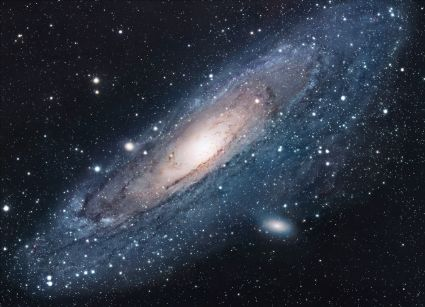
\includegraphics[width=0.7\textwidth]{images/universe.jpg}
\caption{Img example}
\label{fig:universe}
\end{figure}

\begin{figure}[tbh]
\centering
\usetikzlibrary{shapes.multipart,calc, positioning,patterns,backgrounds}
\makeatletter
\newcommand{\gettikzxy}[3]{%
  \tikz@scan@one@point\pgfutil@firstofone#1\relax
  \edef#2{\the\pgf@x}%
  \edef#3{\the\pgf@y}%
}
\makeatother

\begin{tikzpicture}[stack/.style={rectangle split, rectangle split parts=#1,draw, anchor=center},scale=0.65, transform shape]
\node(s)[stack=14]  {
\nodepart{one}   \vdots    % text
\nodepart{two}   \ttfamily sub ecx, 1     % text
\nodepart{three}   \ttfamily jmp 0x75000014     % two
\nodepart{four} \vdots     % three
\nodepart{five}  \ttfamily 0x04000012 % four
\nodepart{six} \vdots
\nodepart{seven} \ttfamily add eax, 4
\nodepart{eight} \ttfamily mov ebx, [esp]
\nodepart{nine} \ttfamily jmp 0x04001000
\nodepart{ten} \vdots
\nodepart{eleven} \ttfamily pop ebp
\nodepart{twelve} \ttfamily push eax
\nodepart{thirteen} \ttfamily jmp 0x03a4a5a6
\nodepart{fourteen} \vdots
};

\node(q)[stack=9, right=2cm of s]  {
\nodepart{one}   \vdots    % text
\nodepart{two}   \ttfamily add eax,4     % two
\nodepart{three}  \ttfamily mov ebx, [esp]     % three
\nodepart{four}  \ttfamily pop ebp % four
\nodepart{five}  \ttfamily push eax
\nodepart{six} \ttfamily sub ecx,1
\nodepart{seven} \ttfamily MessageBox() + 0x14
\nodepart{eight} \ttfamily MessageBox() + 0x18
\nodepart{nine} \vdots
};

% Adding comments and pointers
\draw[<-,>=stealth](s.two west)--+(-20pt,0pt) node[anchor=east, align=left]{\footnotesize \ttfamily 0x03a4a5a6};
\draw[<-,>=stealth](s.five west)--+(-20pt,0pt) node[anchor=east,text width=1.8cm,align=left]{\footnotesize {\ttfamily 0x04000000} \newline IAT entry};
\draw[<-,>=stealth](s.seven west)--+(-20pt,0pt) node[anchor=east, align=left]{\footnotesize \ttfamily 0x04000012};
\draw[<-,>=stealth](s.eleven west)--+(-20pt,0pt) node[anchor=east, align=left]{\footnotesize \ttfamily 0x04010000};
\draw[->,>=stealth, dashed](s.five east) --+(10pt, 0)  --  node[anchor=west] {1} ([shift=({10pt,0})]s.seven east) -- (s.seven east);
\draw[->,>=stealth, dashed](s.eight east) --+(10pt, 0)  --  node[anchor=west] {2} ([shift=({10pt,0})]s.eleven east) -- (s.eleven east);
\draw[->,>=stealth, dashed](s.thirteen east) --+(25pt, 0)  --  node[anchor=west] {3} ([shift=({25pt,0})]s.two east) -- (s.two east);

%Get x and y coordinates of point A
\gettikzxy{(s.three east)}{\ax
}{\ay}
\gettikzxy{(q.seven west)}{\bx}{\by}

\draw[->,>=stealth, dashed](s.three east) -- (\ax+40pt, \ay)  --  node[anchor=west] {4} (\ax+40pt, \by) -- (q.seven west);

\draw[<-,>=stealth](q.two east)--+(+20pt,0pt) node[anchor=west,text width=2cm,align=left]{\footnotesize {\ttfamily 0x75000000} \newline Entry point MessageBox API};


   \begin{pgfonlayer}{background}
       \draw[pattern=vertical lines, pattern color=red!50] (s.two split east) rectangle (s.one split west);
       \draw[pattern=vertical lines, pattern color=red!50] (q.six split east) rectangle (q.five split west);

       \draw[pattern=north west lines, pattern color=yellow!60] (s.eight split east) rectangle (s.six split west);
       \draw[pattern=north west lines, pattern color=yellow!60] (q.text split east) rectangle (q.three split west);


       \draw[pattern=horizontal lines, pattern color=green!60] (s.ten split east) rectangle (s.twelve split west);
       \draw[pattern=horizontal lines, pattern color=green!60] (q.three split east) rectangle (q.five split west);


%       \draw[pattern=dots, pattern color=blue!60] (e.text split west) rectangle (e.two split east);
 %      \draw[pattern=horizontal lines, pattern color=olive!60] (e.two split west) rectangle (e.three split east);
  %     \draw[pattern=vertical lines, pattern color=magenta!60] (e.three split west) rectangle (e.south east);
    \end{pgfonlayer}


\end{tikzpicture}
 \caption{You can use tikz to draw nice memory drawing (example in file \texttt{stack\_representation\_example.pgf}.). Or google draw.  If you use other tools, make sure to have all figure as \texttt{pdf}. Moreover, if you use an external tool, make sure to provide a way to modify the produced images. A link to google draw with correct permission is good enough.}
\label{general-stolen-api}
\end{figure} 


\subsection{Example of code}
Here you can fine an example of how to add some code. It is using the package minted with basic option enabled.
You can write code in place:
\begin{minted}[linenos, bgcolor=black, escapeinside=!!]{python}
import numpy as np
    
def incmatrix(genl1,genl2):
    m = len(genl1)
    n = len(genl2) !\label{myline}!
    M = None #to become the incidence matrix
    VT = np.zeros((n*m,1), int)  #dummy variable
    
    #compute the bitwise xor matrix
    M1 = bitxormatrix(genl1)
    M2 = np.triu(bitxormatrix(genl2),1) 
...
\end{minted}
You can reference to a line
The important line is line \ref{myline}.

You can use an external file and ave the code as listing.
\begin{listing}[ht]
\inputminted[linenos, bgcolor=black, escapeinside=!!]{python}{x.py}
\caption{Example from external file}
\label{listing:3}
\end{listing}

The important line is line \ref{anotherline} of Listing~\ref{listing:3}.

\section{Conclusion}
``I always thought something was fundamentally wrong with the universe'' \citep{adams1995hitchhiker}

\bibliographystyle{plain}
\bibliography{references}
\end{document}
